\label{appendix:dynamics_model}
\section{Fixed Wing Aircraft Dynamics Model}

The following is the nomenclature that will be used to describe the kinematic equations.  Euler angles for pitch $(\theta)$, roll $(\phi)$, and yaw $(\psi)$ will have the units of radians.  The following Figure~\ref{fig:reference_frame} illustrates the \ac{NED} reference frame definitions used for body rotational rates about the $x$ axis $(p)$, $y$ axis $(q)$, and the $z$ axis $(r)$ as well as the body velocities in the $x$ axis $(u)$, $y$ axis $(v)$, and the $z$ axis $(w)$.

\begin{figure}[h!]
 \centering
  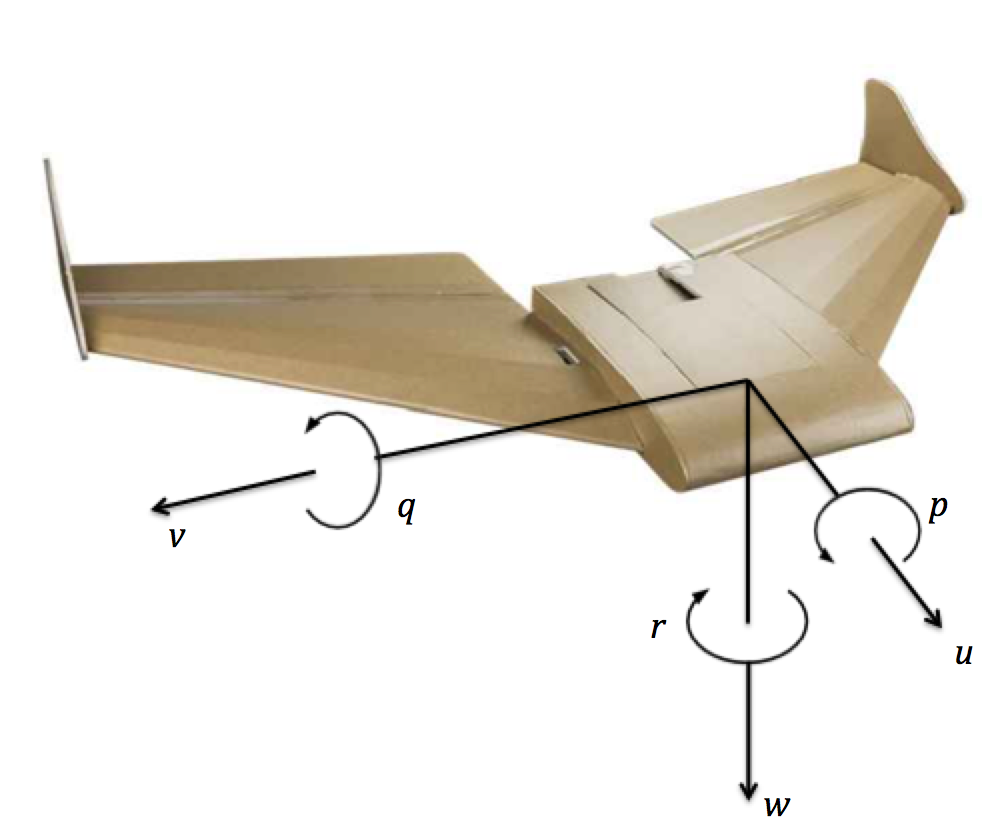
\includegraphics[width=0.65\textwidth]{body_frame_rotations.png}
  \caption{Reference frame - body rates and velocities}
  \label{fig:reference_frame}
\end{figure}

The primary goal of this research is to implement an algorithm which controls fixed wing aircraft attitude.  Therefore, the focus of the following kinematic and dynamics equations will primarily concentrate on deriving only rotational dynamics from first principles.  

Newton's second law as it pertains to rotational motion can be stated as
\begin{equation}\label{eq:rotational_inertia}
\tau=J\frac{d\omega}{dt_i}
\end{equation}

where $\tau$ is the torques applied to the body, $J$ is the moment of inertia, and $ \frac{d\omega}{dt_i}$ is the angular acceleration of the body with respect to the inertial frame.

Equation~\ref{eq:rotational_inertia} can be rewritten in the body reference frame as follows:

\begin{equation}
\tau^b=J\dot{\omega}_{b/i}^b+\omega_{b/i}^b\times\left(J\omega_{b/i}^b\right)
\end{equation}

The expression $\dot{\omega}_{b/i}^b$ is the angular acceleration in the body frame as viewed in the body frame:

\begin{equation}
\dot{\omega}_{b/i}^b=
\begin{pmatrix}
\dot{p}\\
\dot{q}\\
\dot{r}
\end{pmatrix}
\end{equation}

The equation can then be rewritten with respect to $\dot{\omega}_{b/i}^b$:

\begin{equation}
\dot{\omega}_{b/i}^b=J^{-1}\left[-\omega_{b/i}^b\times\left(J\omega_{b/i}^b\right)+\tau^b\right]
\end{equation}

$J$ can be defined as the inertia matrix as follows

\begin{equation}
J=
 \begin{pmatrix}
 J_x & -J_{xy} & -J_{xz}\\
 -J_{xy} & J_y & -J_{yz}\\
 -J_{xz} & -J_{yz} & J_z
 \end{pmatrix}
\end{equation}

The moments of inertia, or the diagonal terms, are always non-zero for any rigid body.  The products of inertia, or the off-diagonal terms, are terms which describe the inertial coupling between axis.  For a traditional fixed wing aircraft, the natural symmetry will simplify the inertia matrix in the off-diagonal terms as follows:

\begin{equation}
J=
 \begin{pmatrix}
 J_x & 0 & -J_{xz}\\
 0 & J_y & 0\\
 -J_{xz} & 0 & J_z
 \end{pmatrix}
\end{equation}

The inverse of $J$ can be found to be

\begin{equation}
J^{-1}=
 \begin{pmatrix}
 \frac{J_z}{\Gamma} & 0 & \frac{J_{xz}}{\Gamma}\\
 0 & \frac{1}{J_y} & 0\\
 \frac{J_{xz}}{\Gamma} & 0 & \frac{J_x}{\Gamma}
 \end{pmatrix}
\end{equation}

where,

\begin{equation}
\Gamma = J_xJ_z-J_{xz}^2
\end{equation}

Aircraft nomenclature for torques are defined $\tau\triangleq(l,m,n)^T$ and therefore the combined equations derived from first principles take the form:

\begin{equation}\label{eq:body_rate_derivation}
\begin{split}
 \begin{pmatrix}
  \dot{p} \\
  \dot{q} \\
  \dot{r} 
 \end{pmatrix}
 &=
 \begin{pmatrix}
 \frac{J_z}{\Gamma} & 0 & \frac{J_{xz}}{\Gamma}\\
 0 & \frac{1}{J_y} & 0\\
 \frac{J_{xz}}{\Gamma} & 0 & \frac{J_x}{\Gamma}
 \end{pmatrix}
 \left[
 \begin{pmatrix}
  0& r& -q \\
  -r& 0& p \\
  q& -p& 0
 \end{pmatrix}
 \begin{pmatrix}
 J_x & 0 & -J_{xz}\\
 0 & J_y & 0\\
 -J_{xz} & 0 & J_z
 \end{pmatrix}
 \begin{pmatrix}
  p\\
  q\\
  r
 \end{pmatrix} +
 \begin{pmatrix}
  l\\
  m\\
  n
 \end{pmatrix}
 \right] \\ 
 &=
 \begin{pmatrix}
  \frac{J_z}{\Gamma} & 0 & \frac{J_{xz}}{\Gamma}\\
  0 & \frac{1}{J_y} & 0\\
  \frac{J_{xz}}{\Gamma} & 0 & \frac{J_x}{\Gamma}
 \end{pmatrix}
 \left[
 \begin{pmatrix}
 J_{xz}pq+(J_y-J_z)qr\\
 J_{xz}(r^2-p^2)+(J_z-J_x)pr\\
 (J_x-J_y)pq-J_{xz}qr
 \end{pmatrix}+
 \begin{pmatrix}
  l\\
  m\\
  n
 \end{pmatrix}
 \right]\\ 
 &=
 \begin{pmatrix}
  \Gamma_1pq-\Gamma_2qr+\Gamma_3l+\Gamma_4n\\
  \Gamma_5pr-\Gamma_6(p^2-r^2)+\frac{1}{J_y}m\\
  \Gamma_7pq-\Gamma_1qr+\Gamma_4l+\Gamma_8n
 \end{pmatrix}
 \end{split}  
\end{equation}
where,

\begin{equation}
\begin{split}
\Gamma_1&=\frac{J_{xz}(J_x-J_y+J_z)}{\Gamma}\\
\Gamma_2&=\frac{J_z(J_z-J_y)+J_{xz}^2}{\Gamma}\\
\Gamma_3&=\frac{J_z}{\Gamma}\\
\Gamma_4&=\frac{J_{xz}}{\Gamma}\\
\Gamma_5&=\frac{J_z-J_x}{J_y}\\
\Gamma_6&=\frac{J_{xz}}{J_y}\\
\Gamma_7&=\frac{J_x(J_x-J_y)+J_{xz}^2}{\Gamma}\\
\Gamma_8&=\frac{J_x}{\Gamma}\\
\end{split}
\end{equation}

The aerodynamic torques (excluding propulsive torques) can be found to be:

\begin{equation}\label{eq:aero_torques}
\begin{pmatrix}
  l\\
  m\\
  n
 \end{pmatrix}
 =
 \frac{1}{2}\rho V_a^2S
 \begin{pmatrix}
  b\left[C_{l_0}+C_{l_\beta}\beta+C_{l_p}\frac{b}{2Va}p+C_{l_r}\frac{b}{2V_a}r+C_{l_{\delta_a}}\delta_a+C_{l_{\delta_r}}\delta_r\right]\\
  c\left[C_{m_0}+C_{m_\alpha}\alpha+C_{m_q}\frac{c}{2V_a}q+C_{m_{\delta_e}}\delta_e\right]\\
  b\left[C_{n_0}+C_{n_\beta}\beta+C_{n_p}\frac{b}{2Va}p+C_{n_r}\frac{b}{2V_a}r+C_{n_{\delta_a}}\delta_a+C_{n_{\delta_r}}\delta_r\right]
 \end{pmatrix}
\end{equation}

Substituting the aerodynamic torques found in Equation~\ref{eq:aero_torques} into Equation~\ref{eq:body_rate_derivation} results in \cite{beard2012small}:
\begin{equation}\label{eq:body_rate_equations}
\begin{split}
 \dot{p}&=\Gamma_1pq-\Gamma_2qr+\frac{1}{2}\rho V_a^2Sb\left[C_{p_0}+C_{p_\beta}\beta+C_{p_p}\frac{bp}{2V_a}+C_{p_r}\frac{br}{2V_a}+C_{p_{\delta_a}}\delta_a+C_{p_{\delta_r}}\delta_r\right]\\
 \dot{q}&=\Gamma_5pr-\Gamma_6(p^2-r^2)+\frac{1}{2}\rho V_a^2Sc\frac{1}{J_y}\left[C_{m_0}+C_{m_\alpha}\alpha+C_{m_q}\frac{cq}{2V_a}+C_{m_{\delta_e}}\delta_e\right]\\
 \dot{r}&=\Gamma_7pq-\Gamma_1qr+\frac{1}{2}\rho V_a^2Sb\left[C_{r_0}+C_{r_\beta}\beta+C_{r_p}\frac{bp}{2V_a}+C_{r_r}\frac{br}{2V_a}+C_{r_{\delta_a}}\delta_a+C_{r_{\delta_r}}\delta_r\right]
\end{split} 
\end{equation}

Simplifying Equation~\ref{eq:body_rate_equations} assuming no inertial or aerodynamic coupling results in:

\begin{equation}\label{eq:body_rate_simplified}
\begin{split}
 \dot{p}&=\frac{1}{2}\rho V_a^2Sb\left[C_{p_{\delta_a}}\delta_a+C_{p_p}\frac{bp}{2V_a}+C_{p_0}\right]\\
 \dot{q}&=\frac{1}{2}\rho V_a^2Sc\frac{1}{J_y}\left[C_{m_{\delta_e}}\delta_e+C_{m_q}\frac{cq}{2V_a}+C_{m_0}\right]\\
 \dot{r}&=\frac{1}{2}\rho V_a^2Sb\left[C_{r_{\delta_r}}\delta_r+C_{r_r}\frac{br}{2V_a}+C_{r_0}\right]
\end{split} 
\end{equation}

The equations in Equation~\ref{eq:body_rate_simplified} are then slightly modified to fit the first order \ac{ODE} model as described in Equation~\ref{eq:state_space_model}.
\begin{equation}\label{eq:simplified_ac_model}
\begin{split}
\dot{p}&=A_p\hat{p}+b_p\left(\hat{\omega}_p\delta_a+\hat{\theta}_pp+\hat{\sigma}_p\right)\\
\dot{q}&=A_q\hat{q}+b_q\left(\hat{\omega}_q\delta_e+\hat{\theta}_qq+\hat{\sigma}_q\right)\\
\dot{r}&=A_r\hat{r}+b_r\left(\hat{\omega}_r\delta_r+\hat{\theta}_rr+\hat{\sigma}_r\right)
\end{split}
\end{equation}
where the parameters are as follows,
\begin{itemize}
 \item[] $\omega$ - input gain coefficient
 \item[] $\theta$ - constant state coefficient
 \item[] $\sigma$ - disturbance estimate
\end{itemize}

